Abbildungen der Messreihen mit Sendespannungen von 5\,V und 10\,V bei Abständen von ein bis fünf Metern.\\
\begin{minipage}{0.46\textwidth}
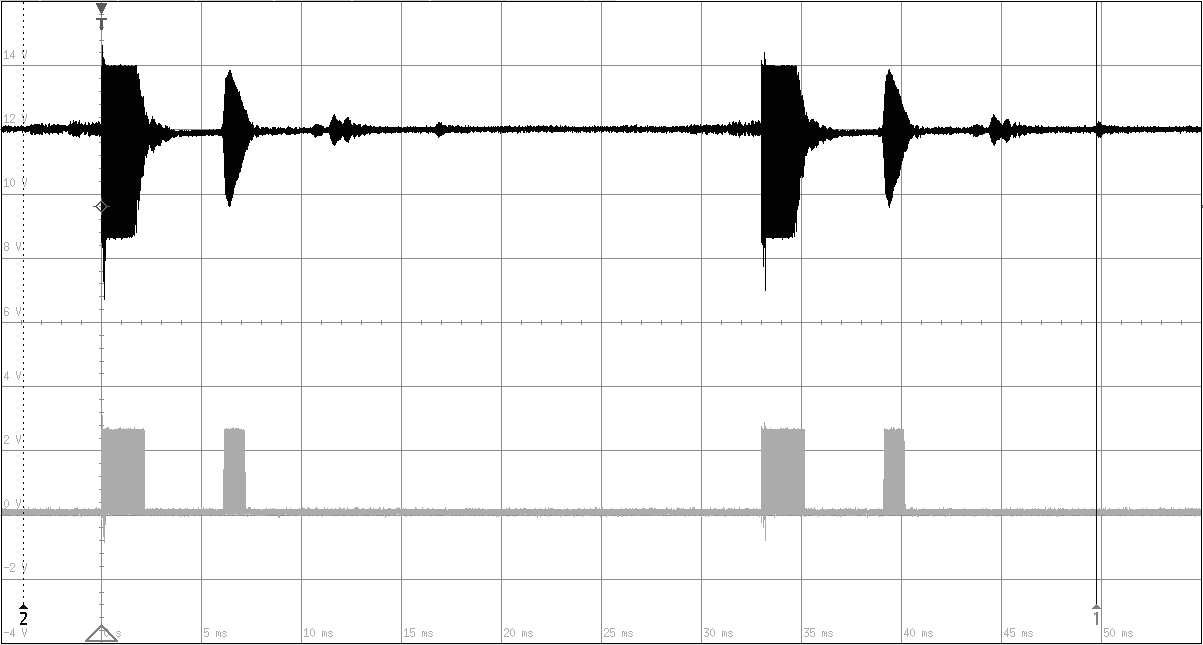
\includegraphics[width=1\textwidth%, draft
]{Abbildungen/MessungenP2/5V/1m.PNG}
\captionof{figure}{Signalverlauf bei 5\,V auf 1\,m Abstand}
\end{minipage}\qquad
\begin{minipage}{0.46\textwidth}
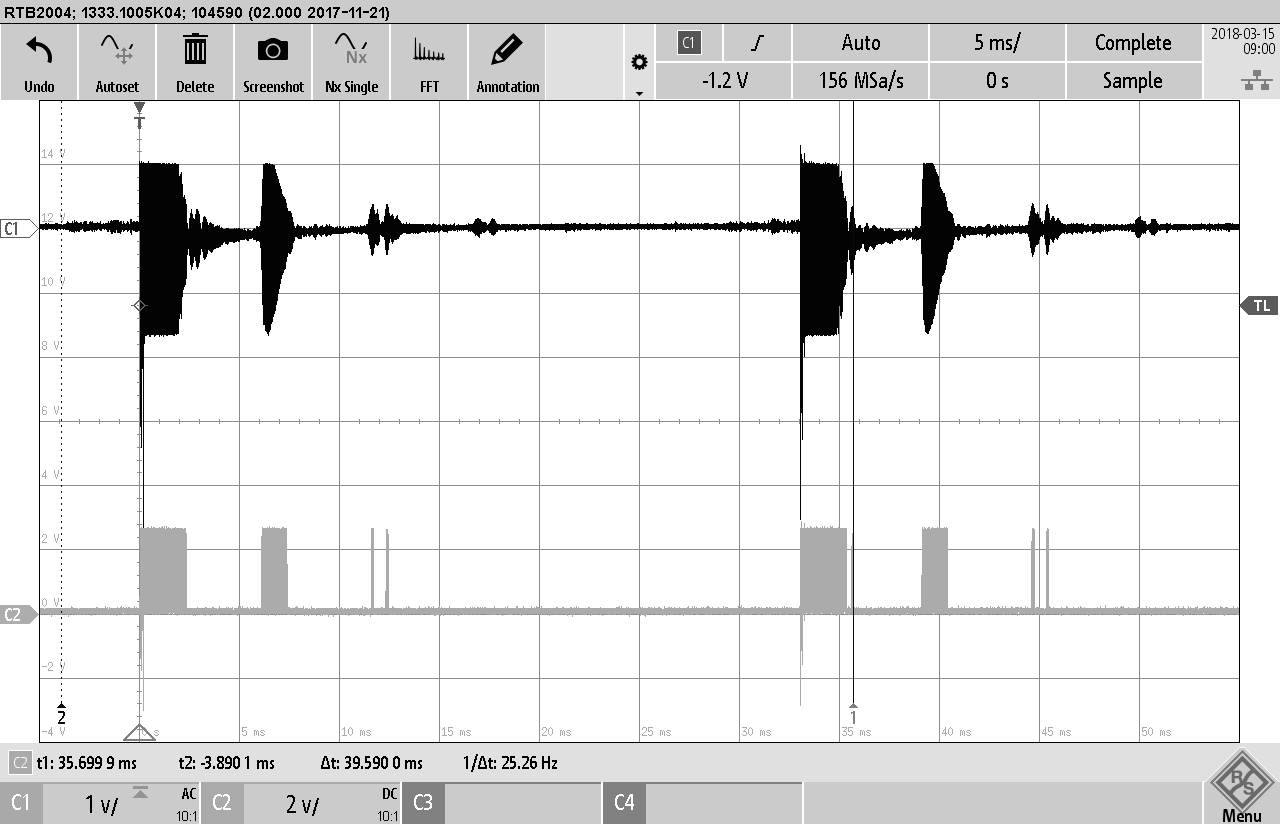
\includegraphics[width=1\textwidth%, draft
]{Abbildungen/MessungenP2/10V/1m.PNG}
\captionof{figure}{Signalverlauf bei 10\,V auf 1\,m Abstand}
\end{minipage}\\
\begin{minipage}{0.46\textwidth}
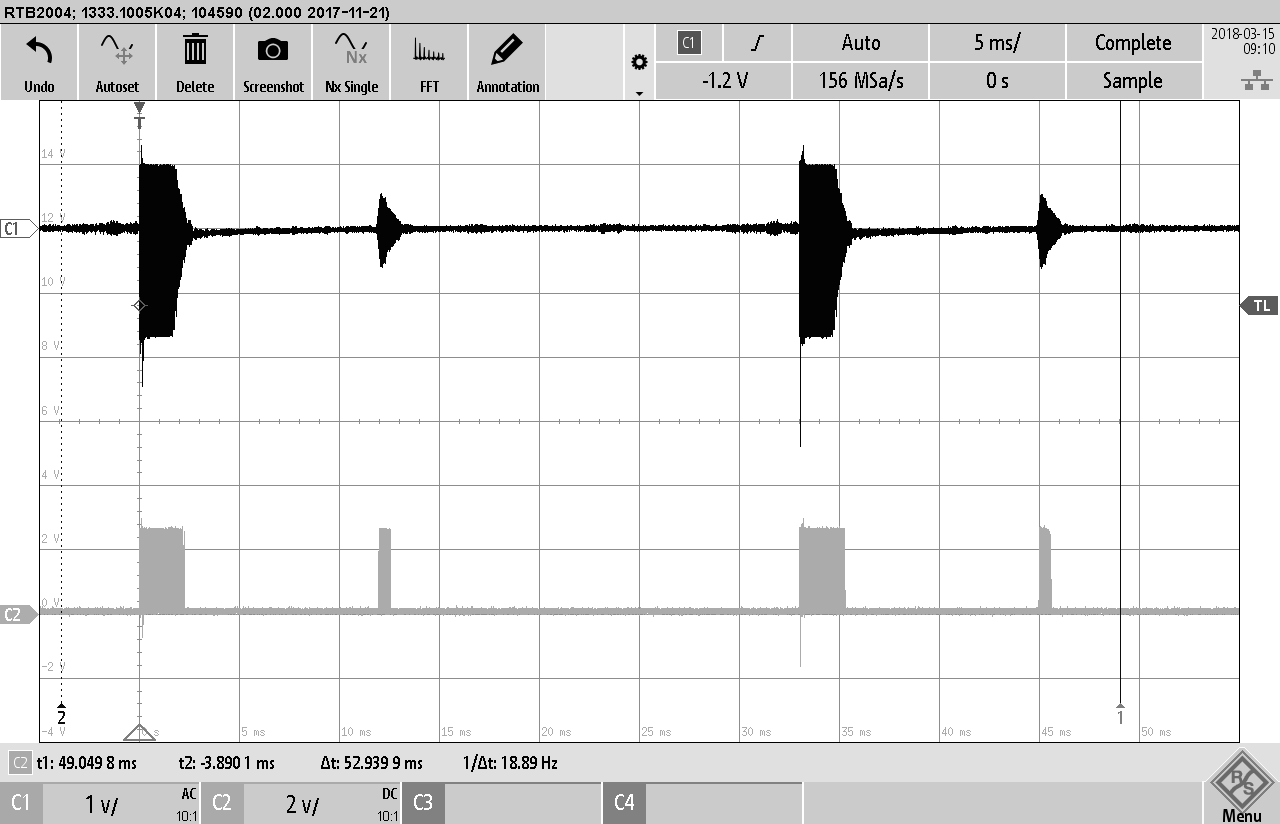
\includegraphics[width=1\textwidth%, draft
]{Abbildungen/MessungenP2/5V/2m.PNG}
\captionof{figure}{Signalverlauf bei 5\,V auf 2\,m Abstand}
\end{minipage}\qquad
\begin{minipage}{0.46\textwidth}
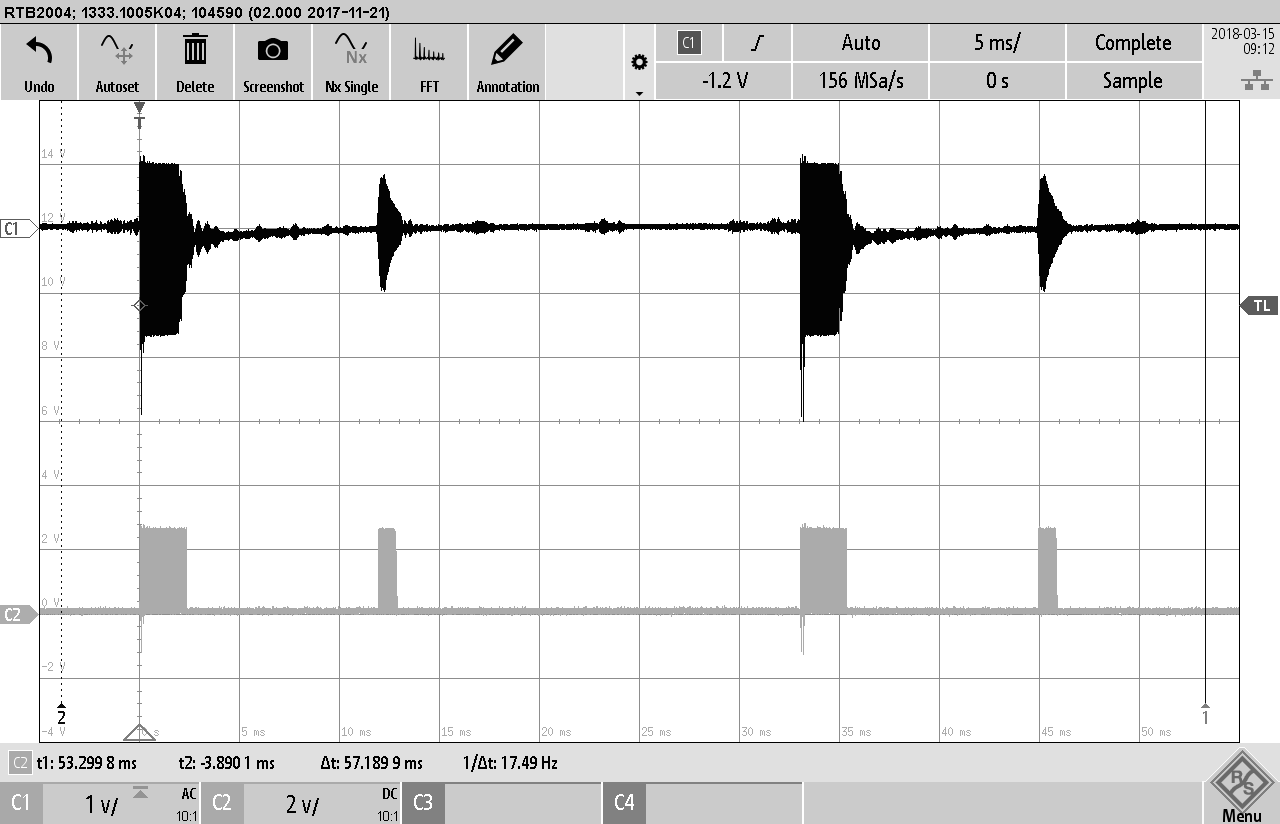
\includegraphics[width=1\textwidth%, draft
]{Abbildungen/MessungenP2/10V/2m.PNG}
\captionof{figure}{Signalverlauf bei 10\,V auf 2\,m Abstand}
\end{minipage}\\
\begin{minipage}{0.46\textwidth}
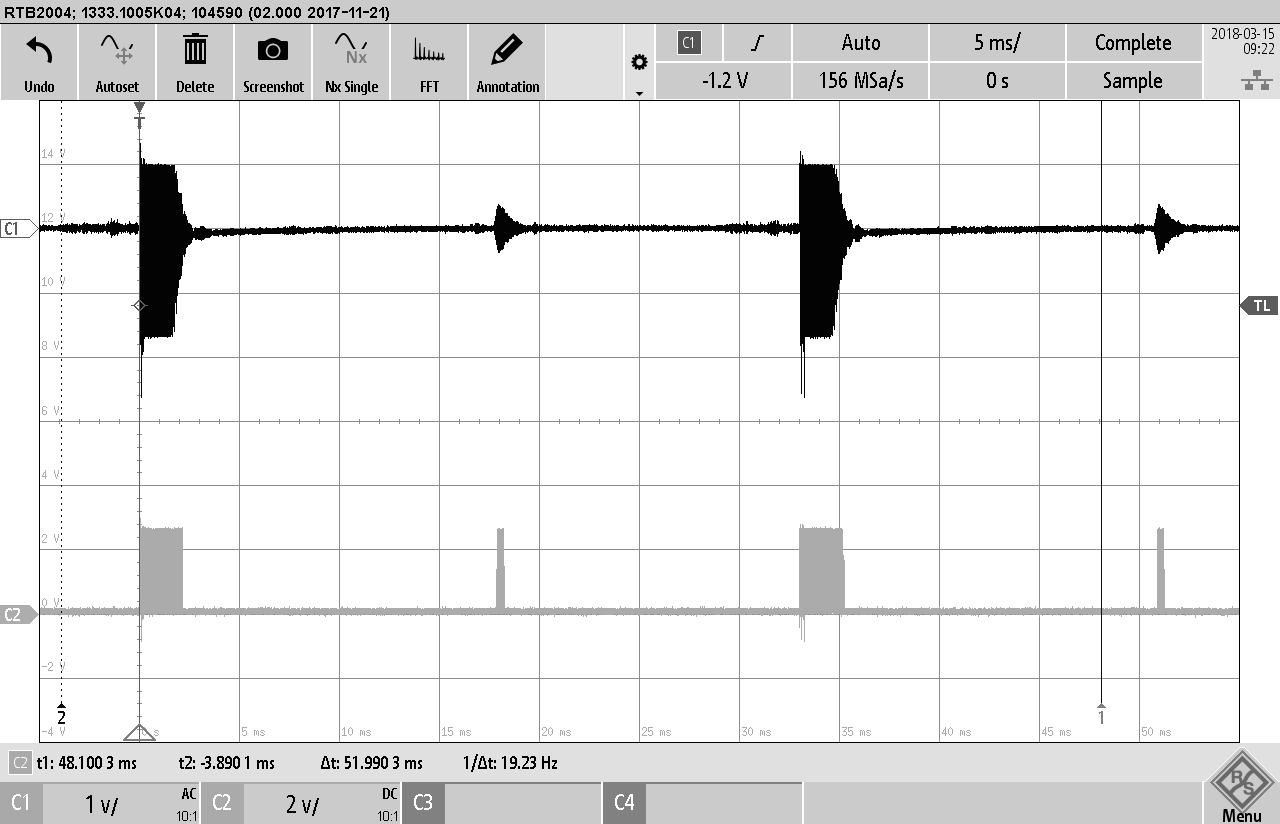
\includegraphics[width=1\textwidth%, draft
]{Abbildungen/MessungenP2/5V/3m.PNG}
\captionof{figure}{Signalverlauf bei 5\,V auf 3\,m Abstand}
\end{minipage}\qquad
\begin{minipage}{0.46\textwidth}
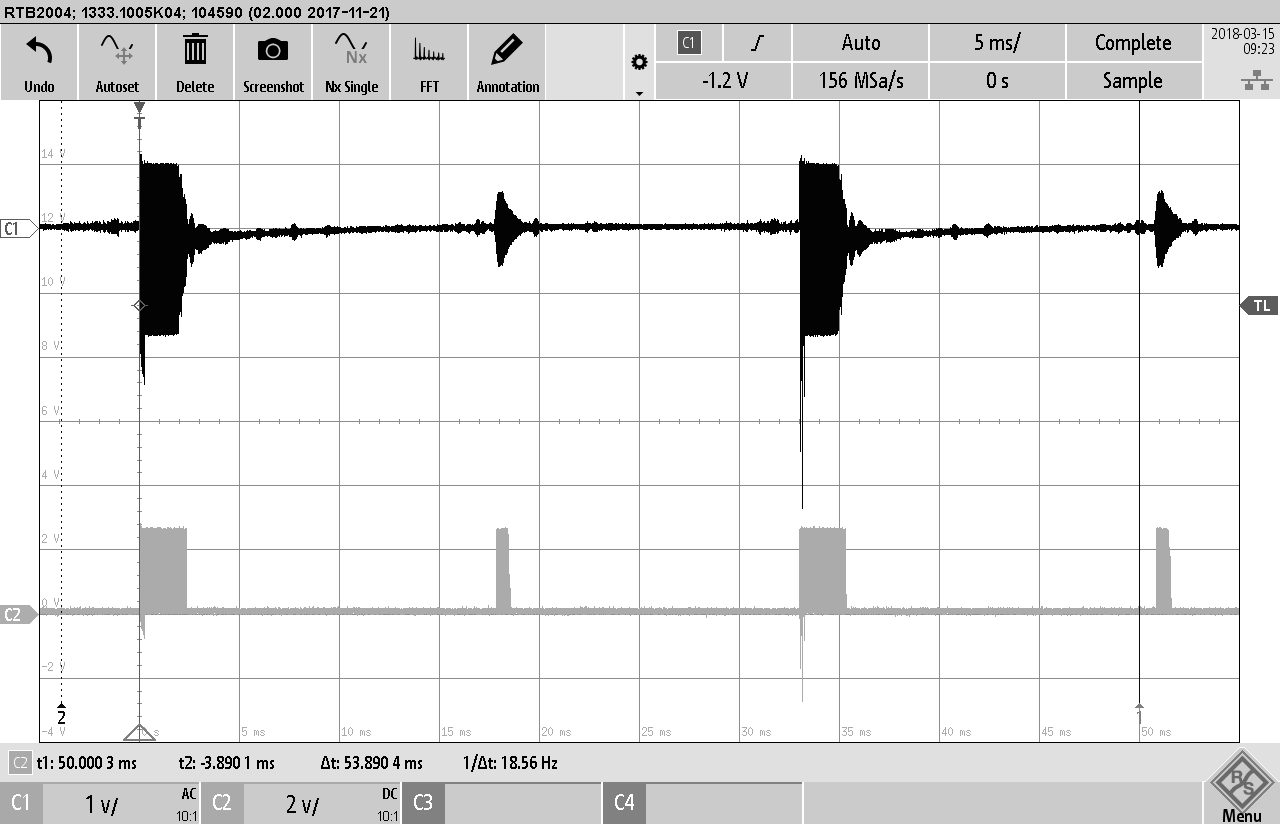
\includegraphics[width=1\textwidth%, draft
]{Abbildungen/MessungenP2/10V/3m.PNG}
\captionof{figure}{Signalverlauf bei 10\,V auf 3\,m Abstand}
\end{minipage}\\
\begin{minipage}{0.46\textwidth}
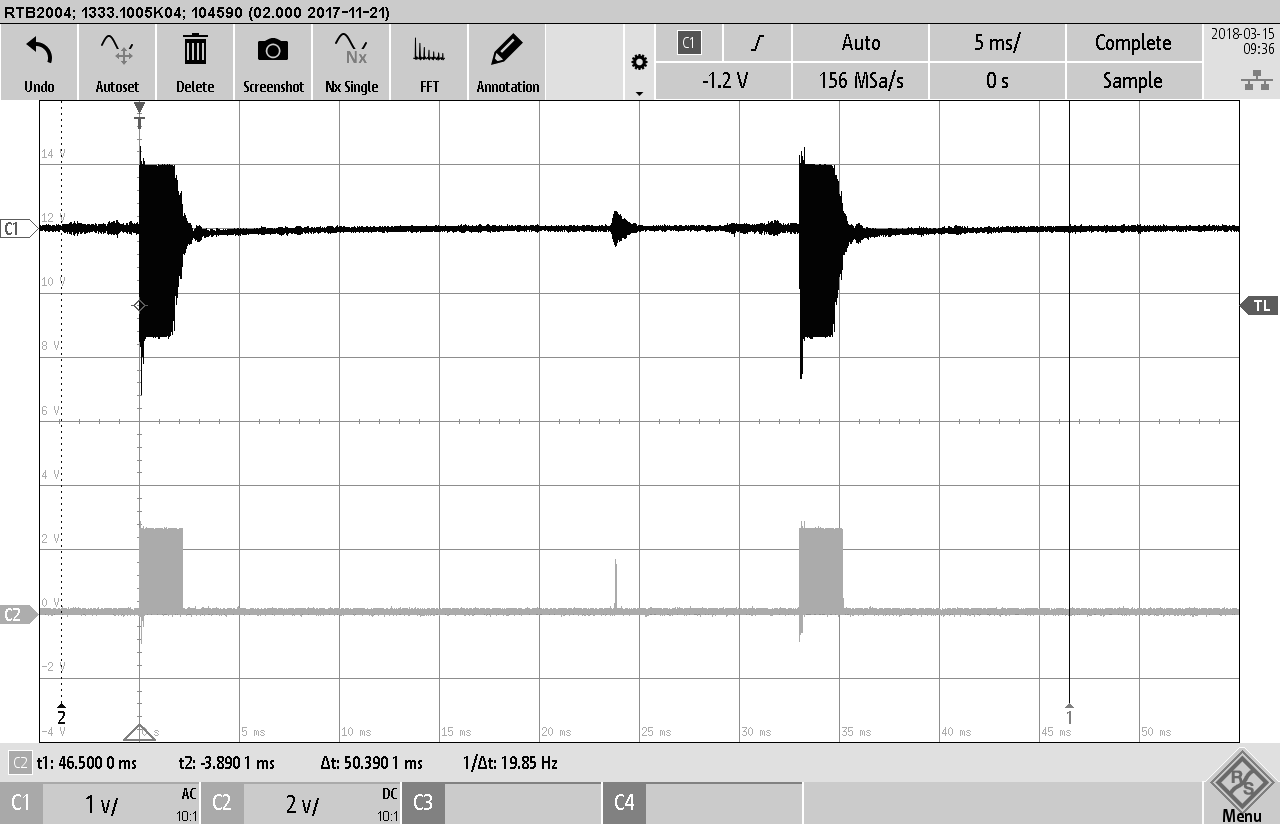
\includegraphics[width=1\textwidth%, draft
]{Abbildungen/MessungenP2/5V/4m.PNG}
\captionof{figure}{Signalverlauf bei 5\,V auf 4\,m Abstand}
\end{minipage}\qquad
\begin{minipage}{0.46\textwidth}
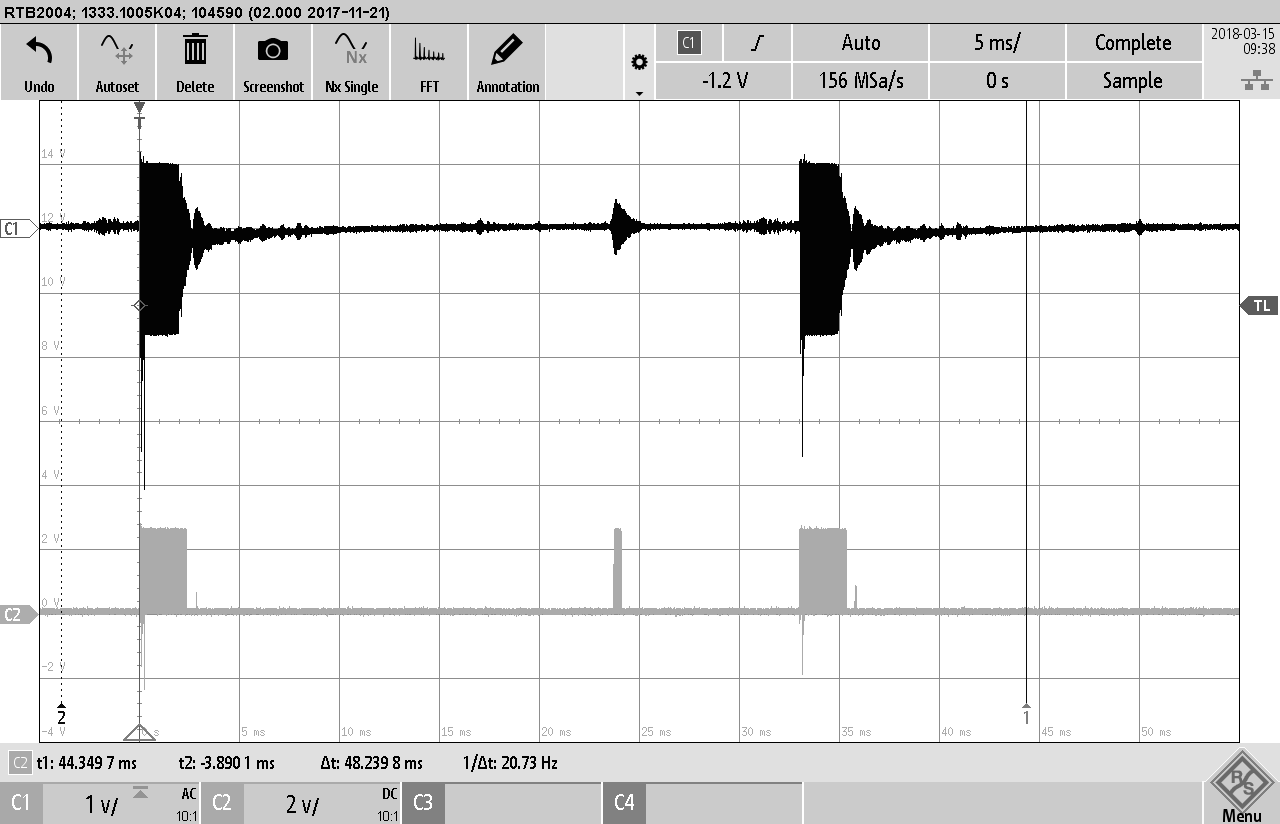
\includegraphics[width=1\textwidth%, draft
]{Abbildungen/MessungenP2/10V/4m.PNG}
\captionof{figure}{Signalverlauf bei 10\,V auf 4\,m Abstand}
\end{minipage}\\
\begin{minipage}{0.46\textwidth}
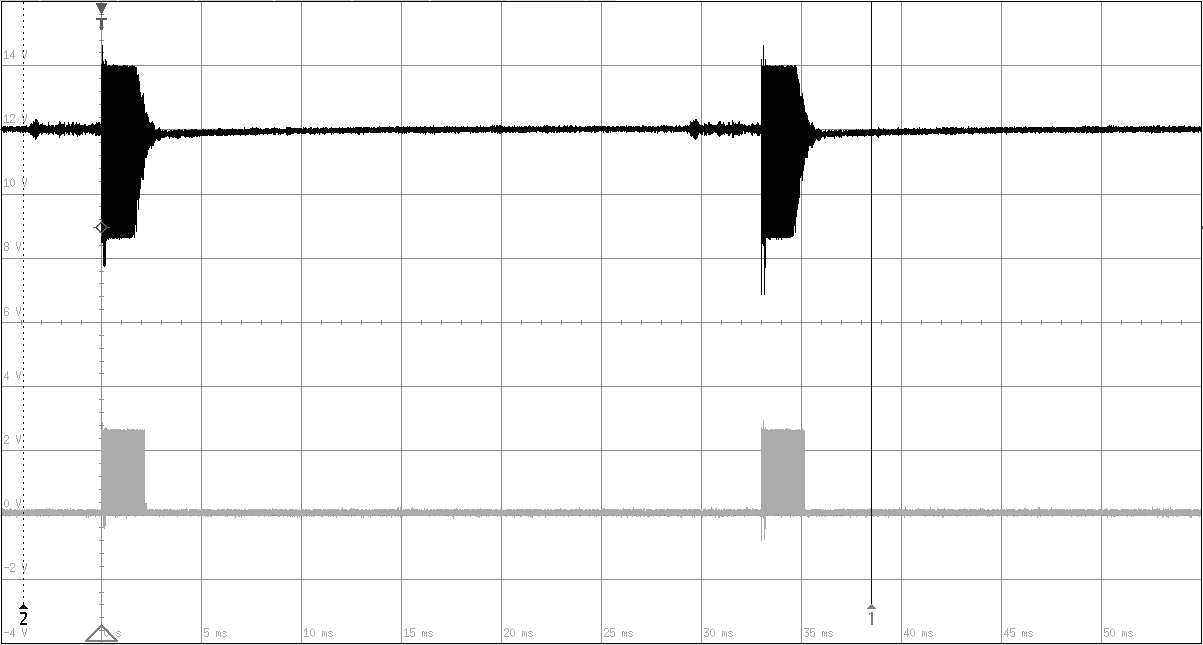
\includegraphics[width=1\textwidth%, draft
]{Abbildungen/MessungenP2/5V/5m.PNG}
\captionof{figure}{Signalverlauf bei 5\,V auf 5\,m Abstand}
\end{minipage}\qquad
\begin{minipage}{0.46\textwidth}
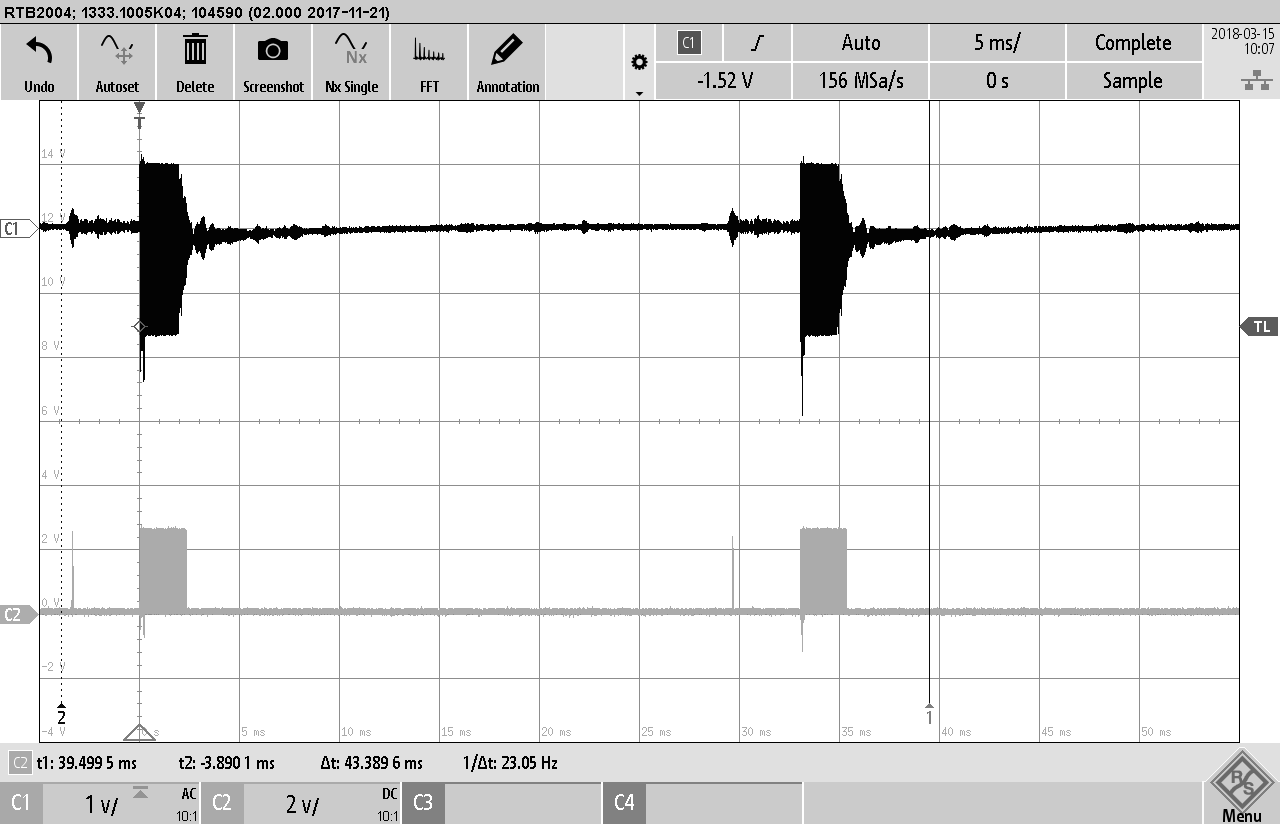
\includegraphics[width=1\textwidth%, draft
]{Abbildungen/MessungenP2/10V/5m.PNG}
\captionof{figure}{Signalverlauf bei 10\,V auf 5\,m Abstand}
\end{minipage}\\
Abbildungen der Messreihen mit Sendespannungen von 15\,V und 20\,V bei Abständen von ein bis fünf Metern.\\
\begin{minipage}{0.46\textwidth}
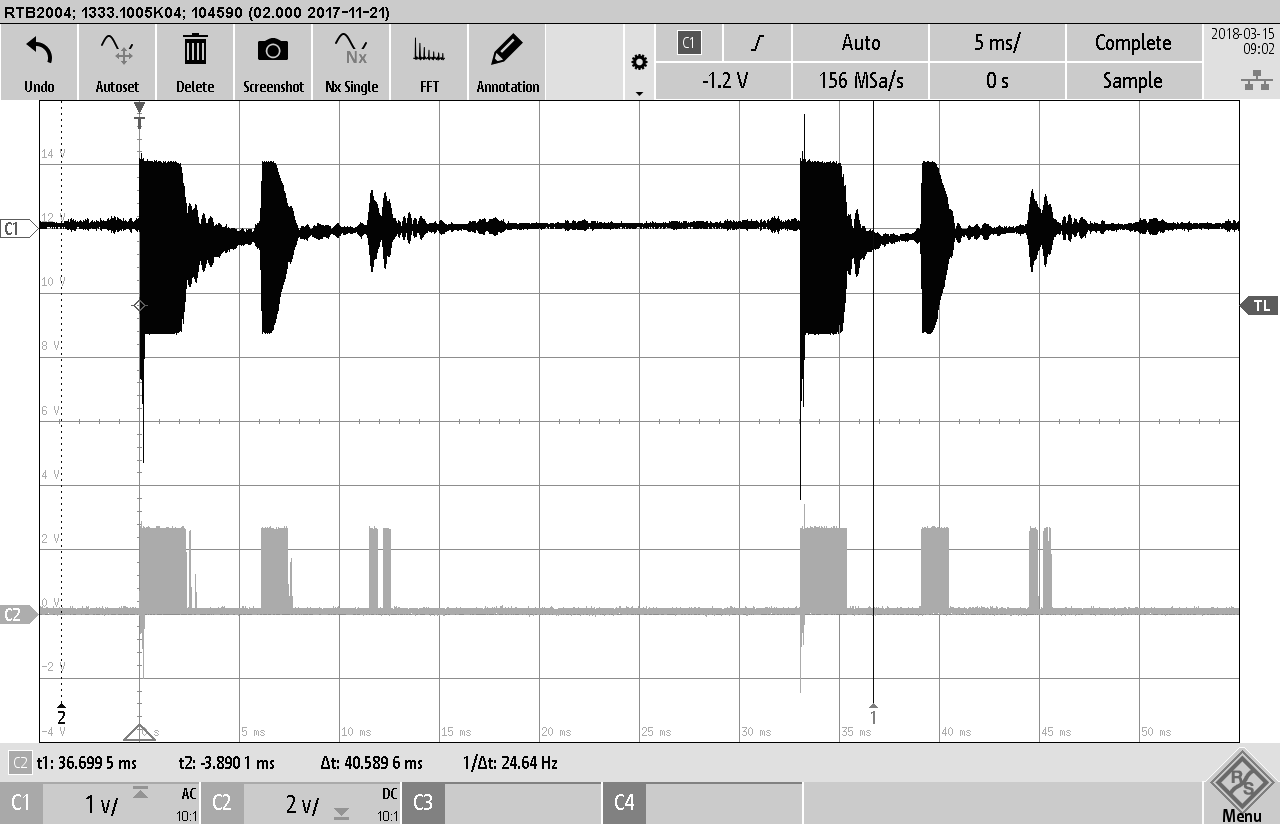
\includegraphics[width=1\textwidth%, draft
]{Abbildungen/MessungenP2/15V/1m.PNG}
\captionof{figure}{Signalverlauf bei 15V auf 1m Abstand}
\end{minipage}\qquad
\begin{minipage}{0.46\textwidth}
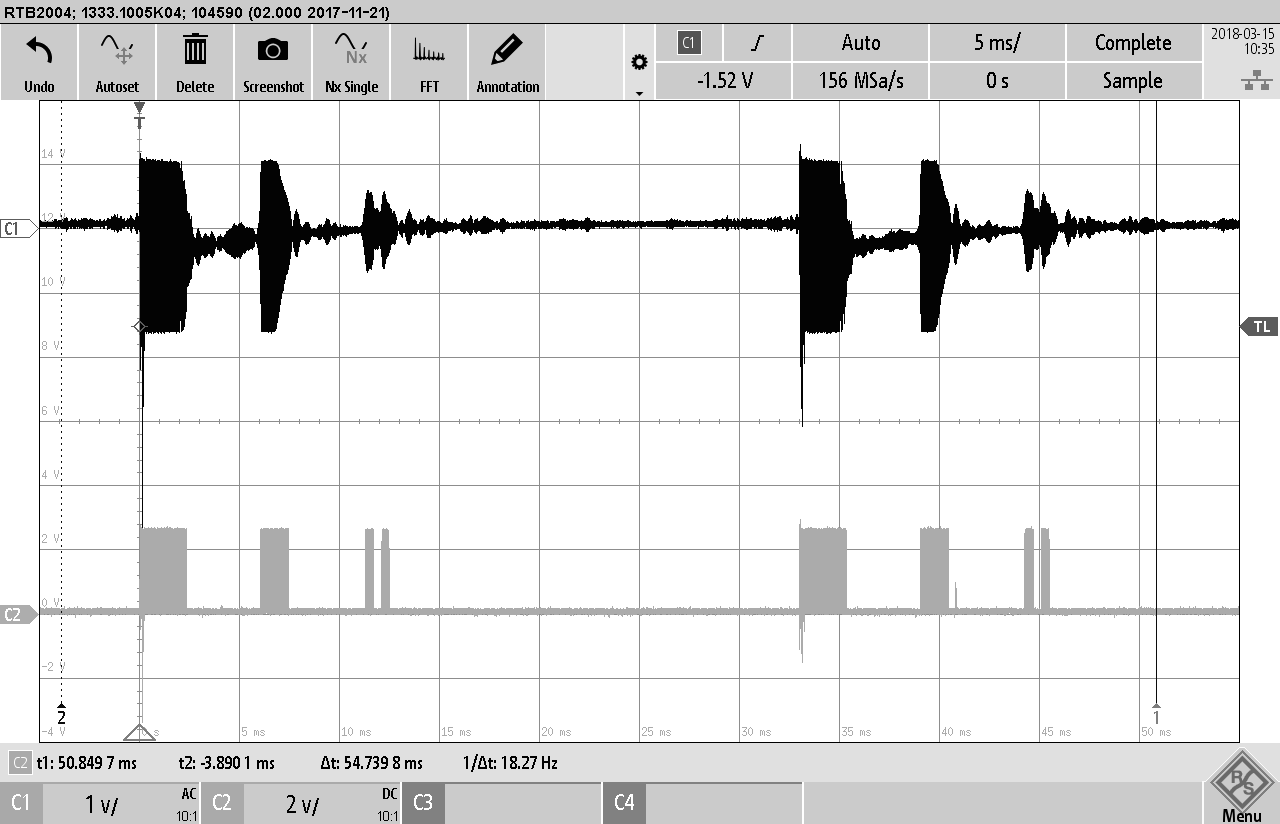
\includegraphics[width=1\textwidth%, draft
]{Abbildungen/MessungenP2/20V/1m.PNG}
\captionof{figure}{Signalverlauf bei 20\,V auf 1\,m Abstand}
\end{minipage}\\
\begin{minipage}{0.46\textwidth}
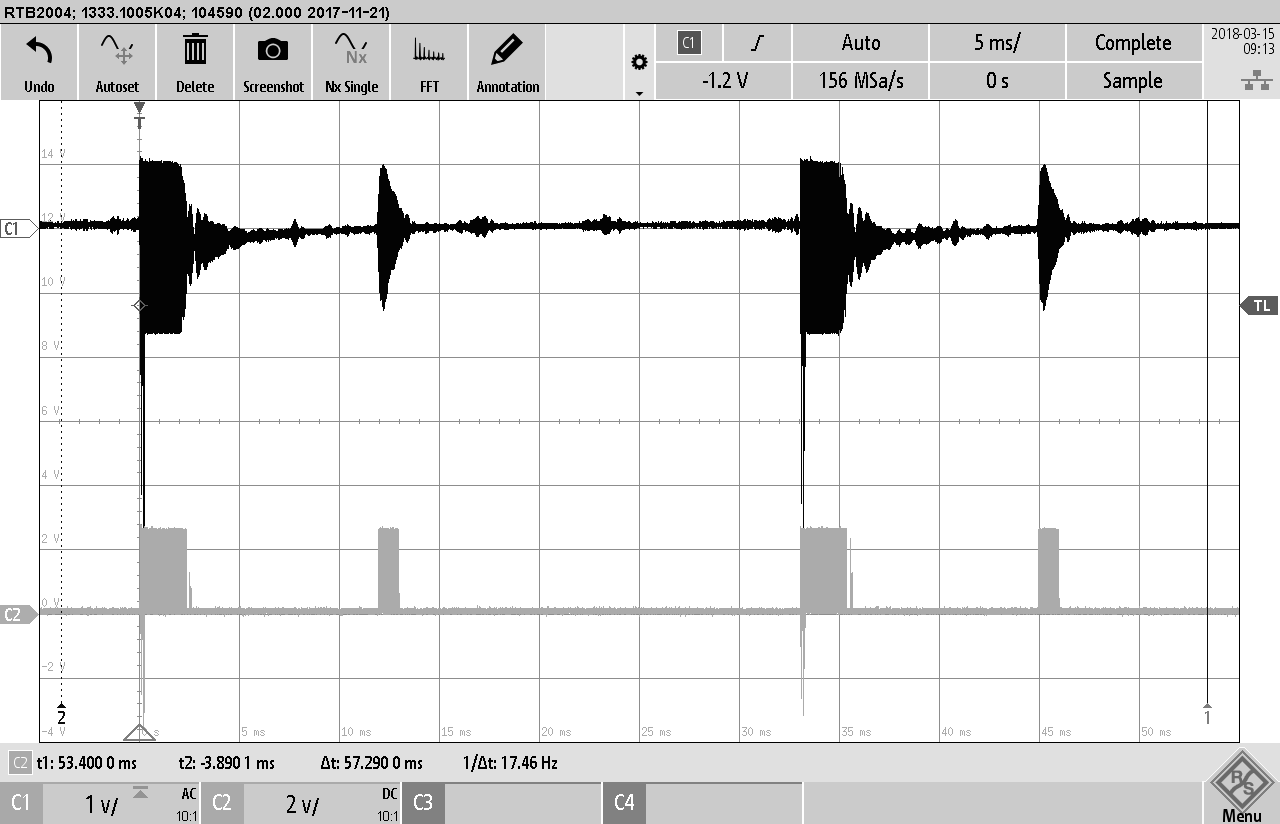
\includegraphics[width=1\textwidth%, draft
]{Abbildungen/MessungenP2/15V/2m.PNG}
\captionof{figure}{Signalverlauf bei 15\,V auf 2\,m Abstand}
\end{minipage}\qquad
\begin{minipage}{0.46\textwidth}
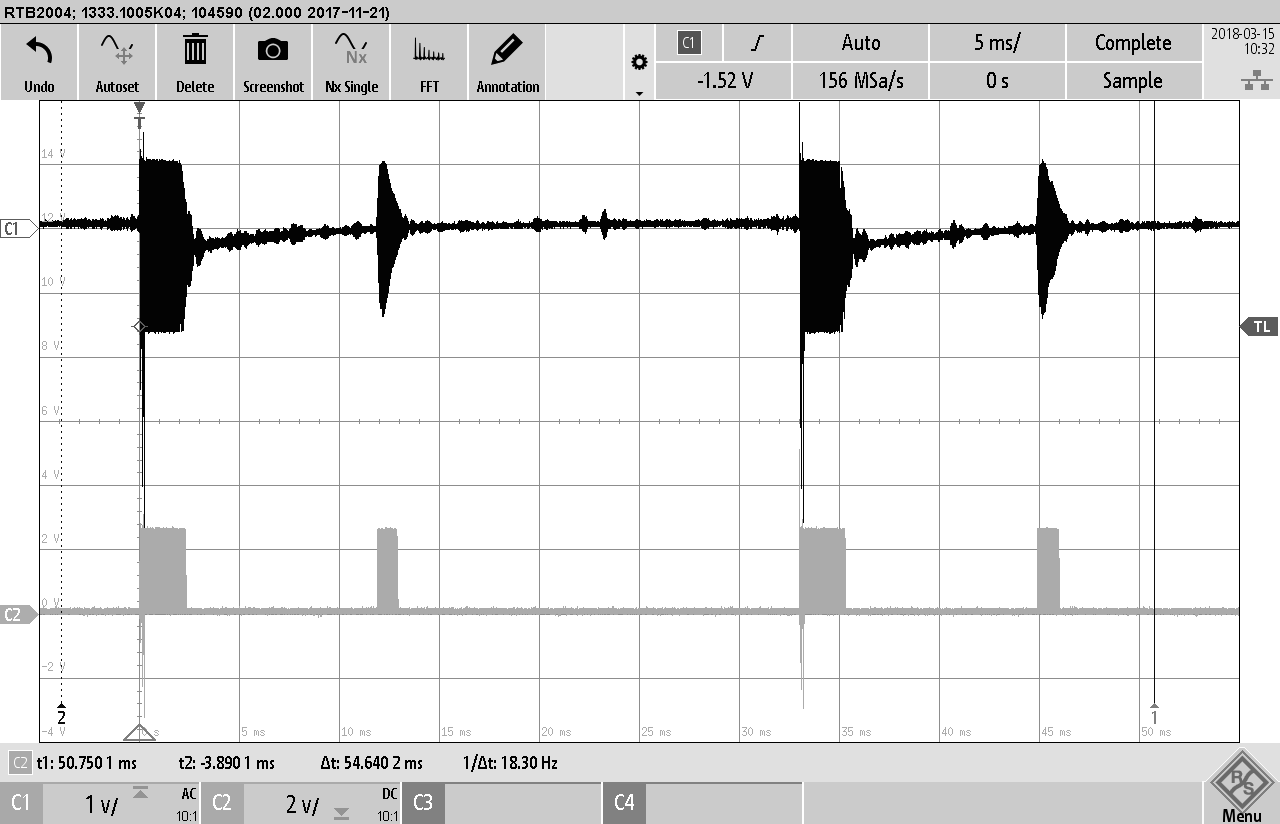
\includegraphics[width=1\textwidth%, draft
]{Abbildungen/MessungenP2/20V/2m.PNG}
\captionof{figure}{Signalverlauf bei 20\,V auf 2\,m Abstand}
\end{minipage}\\
\begin{minipage}{0.46\textwidth}
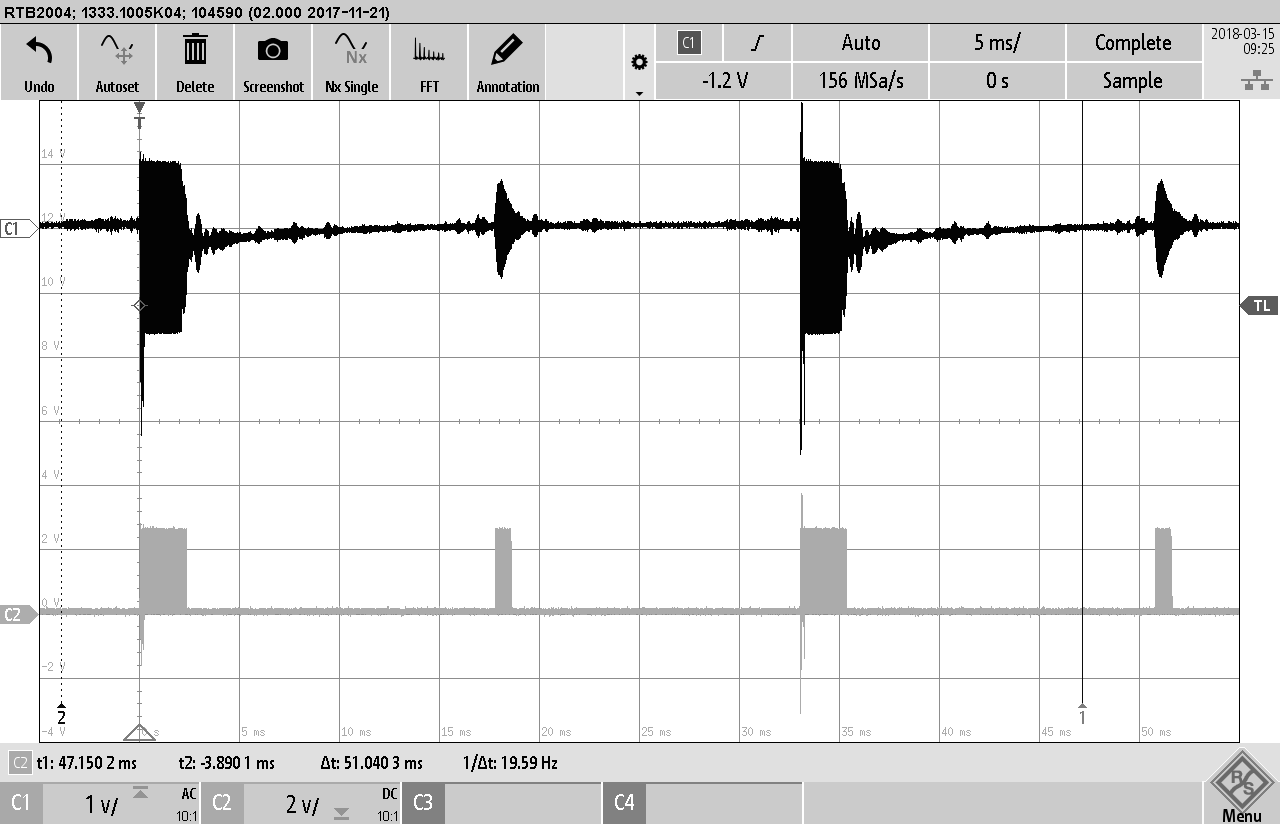
\includegraphics[width=1\textwidth%, draft
]{Abbildungen/MessungenP2/15V/3m.PNG}
\captionof{figure}{Signalverlauf bei 15\,V auf 3\,m Abstand}
\end{minipage}\qquad
\begin{minipage}{0.46\textwidth}
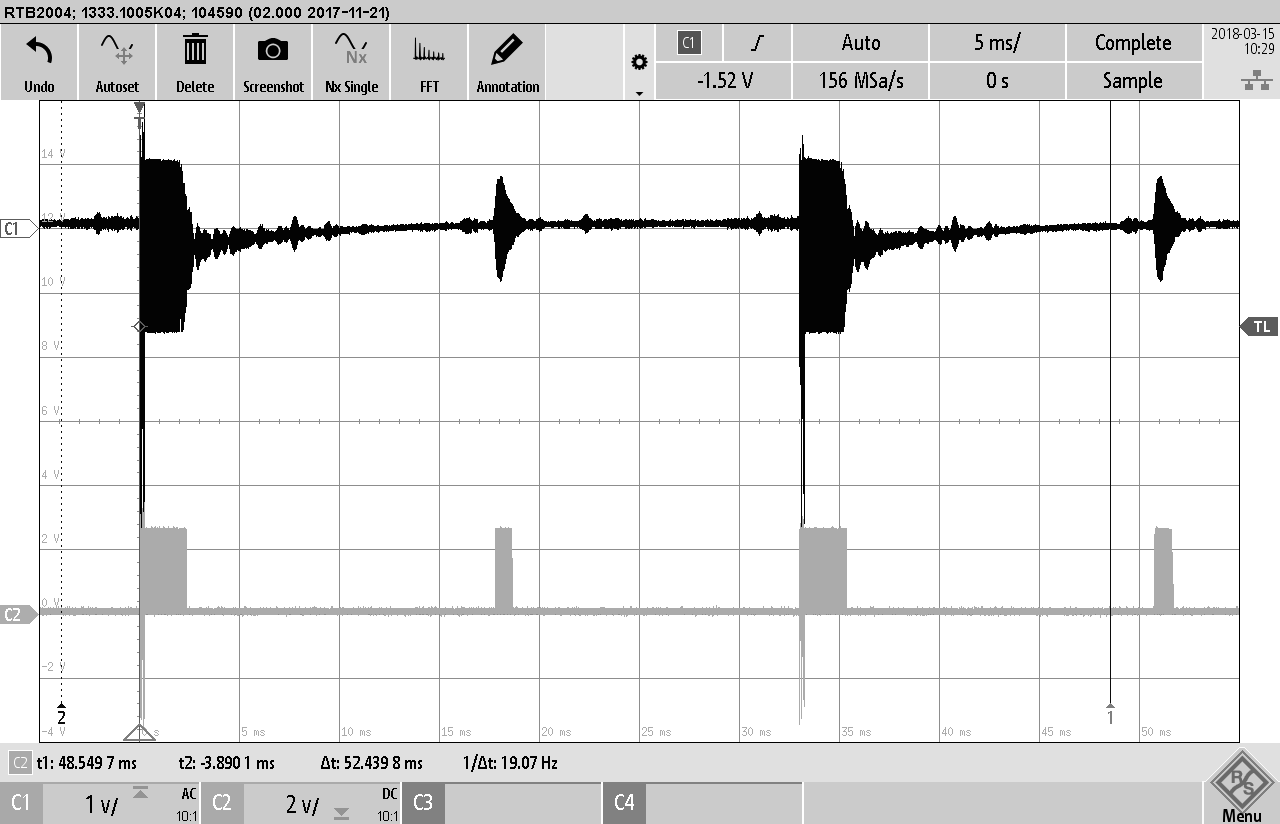
\includegraphics[width=1\textwidth%, draft
]{Abbildungen/MessungenP2/20V/3m.PNG}
\captionof{figure}{Signalverlauf bei 20V auf 3m Abstand}
\end{minipage}\\
\begin{minipage}{0.46\textwidth}
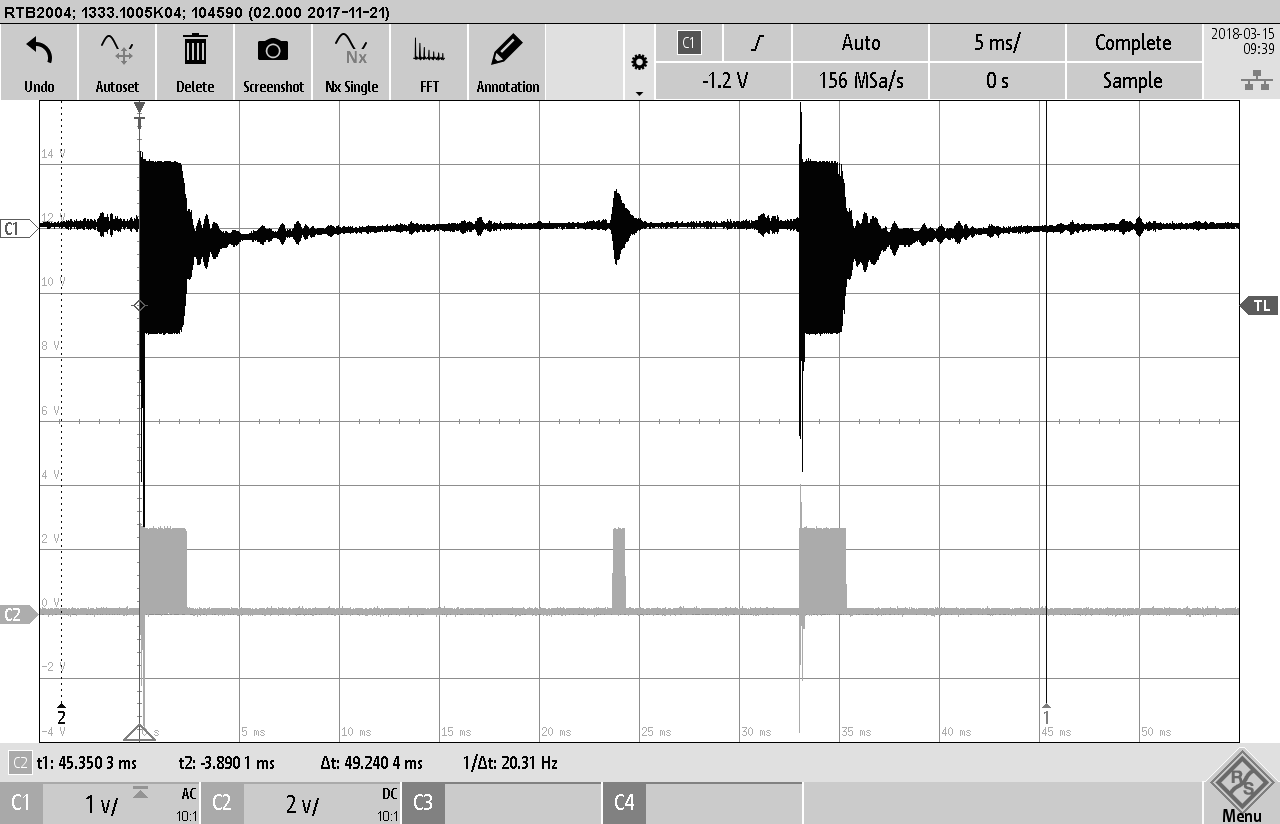
\includegraphics[width=1\textwidth%, draft
]{Abbildungen/MessungenP2/15V/4m.PNG}
\captionof{figure}{Signalverlauf bei 15\,V auf 4\,m Abstand}
\end{minipage}\qquad
\begin{minipage}{0.46\textwidth}
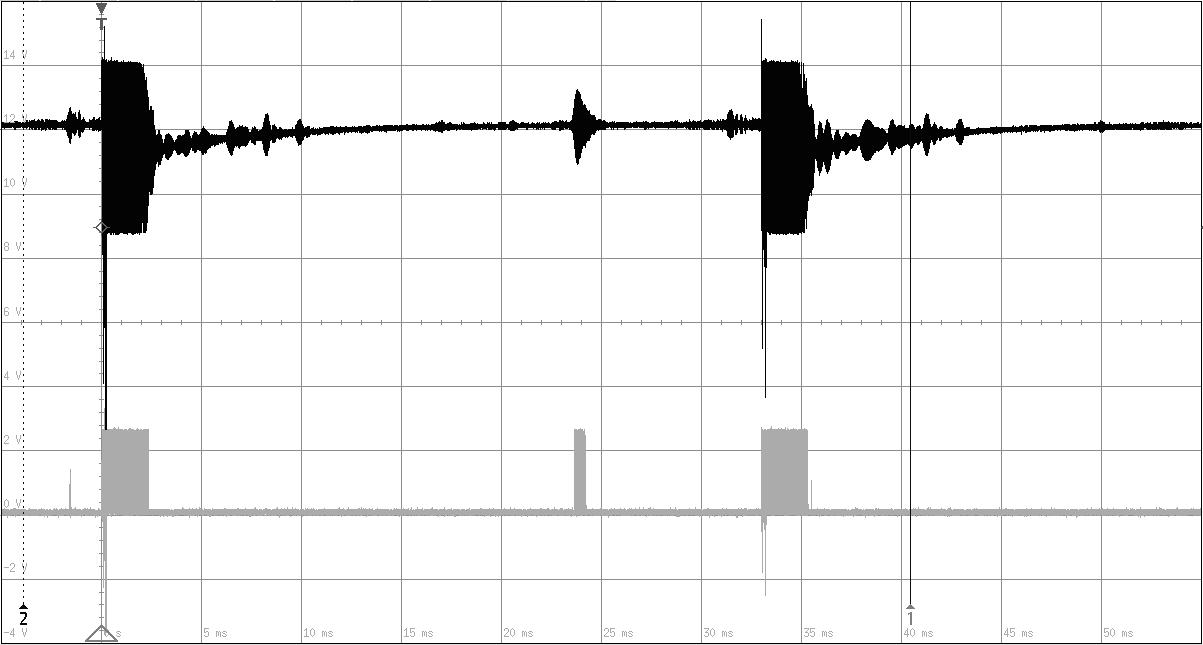
\includegraphics[width=1\textwidth%, draft
]{Abbildungen/MessungenP2/20V/4m.PNG}
\captionof{figure}{Signalverlauf bei 20\,V auf 4\,m Abstand}
\end{minipage}\\
\begin{minipage}{0.46\textwidth}
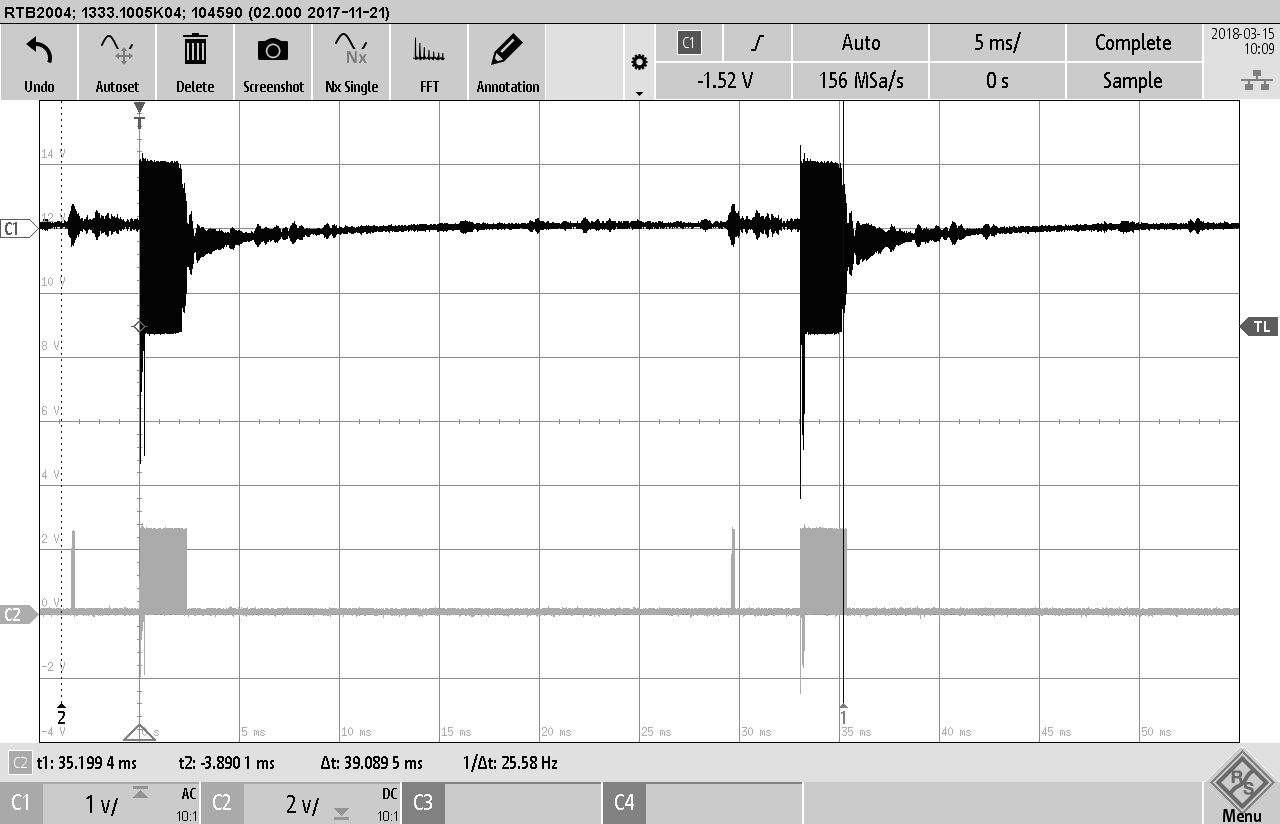
\includegraphics[width=1\textwidth%, draft
]{Abbildungen/MessungenP2/15V/5m.PNG}
\captionof{figure}{Signalverlauf bei 15\,V auf 5\,m Abstand}
\end{minipage}\qquad
\begin{minipage}{0.46\textwidth}
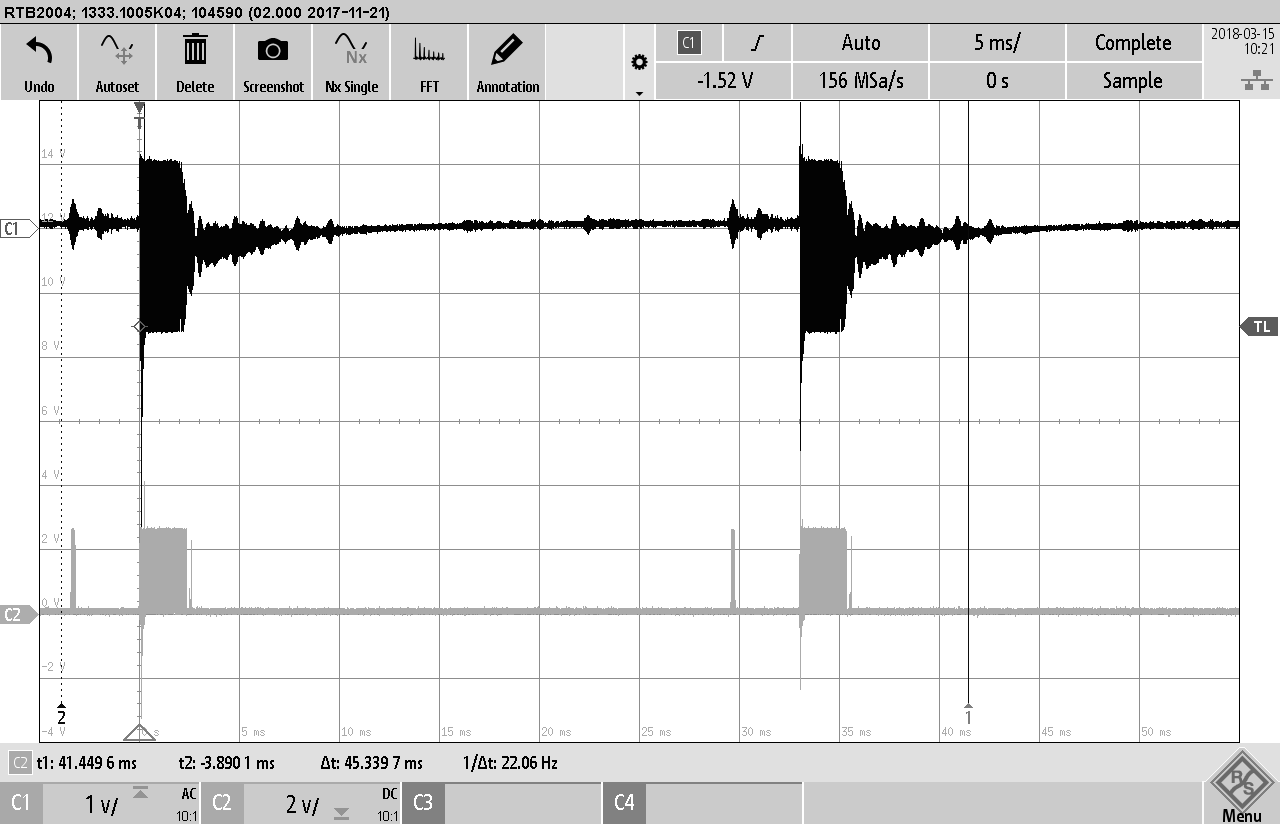
\includegraphics[width=1\textwidth%, draft
]{Abbildungen/MessungenP2/20V/5m.PNG}
\captionof{figure}{Signalverlauf bei 20\,V auf 5\,m Abstand}
\end{minipage}\\
\newpage
Tabellen mit errechneten Objektabständen zu den durchgeführten Messungen\\
\begin{minipage}{1\textwidth}
\captionof{table}{Entfernungsmessung bei 5\,V Sendespannung}
\label{tab:Entfernungsmessung5V}
\begin{tabularx}{\textwidth}{|p{0.1\textwidth}|p{0.2\textwidth}|p{0.2\textwidth}|p{0.2\textwidth}|X|}
\hline
Entfernung [m]& Zeit bis Anfang Echo [ms] & Zeit bis Ende Echo [ms] & Errechnete Entfernung Anfang [m] & Errechnete Entfernung Ende [m]\\
\hline
1 & 6,11 & 7,23 & 1,0485 & 1,2407\\
\hline
1,5 & 9,02 & 9,89 & 1,5478 & 1,6971\\
\hline
2 & 11,97 & 12,76 & 2,0541 & 2,1896\\
\hline
2,5 & 14,88 & 15,5 & 2,5534 & 2,659\\
\hline
3 & 17,84 & 18,2 & 3,06134 & 3,1231\\
\hline
3,5 & 20,8 & 21,11 & 3,569 & 3,6225\\
\hline
4 & 23,71 & 23,81 & 4,0686 & 4,0858\\
\hline
4,5 & 26,61 & 26,73 & 4,5663 & 4,5869\\
\hline
5 & 29,59 & 29,68 & 5,0776 & 5,0961\\
\hline
\end{tabularx}
\end{minipage}
\begin{minipage}{1\textwidth}
\captionof{table}{Entfernungsmessung bei 10\,V Sendespannung}
\label{tab:Entfernungsmessung10V}
\begin{tabularx}{\textwidth}{|p{0.1\textwidth}|p{0.2\textwidth}|p{0.2\textwidth}|p{0.2\textwidth}|X|}
\hline
Entfernung [m]& Zeit bis Anfang Echo [ms] & Zeit bis Ende Echo [ms] & Errechnete Entfernung Anfang [m] & Errechnete Entfernung Ende [m]\\
\hline
1 & 6,07 & 7,37 & 1,0416 & 1,2647\\
\hline
1,5 & 8,99 & 10,02 & 1,5427 & 1,7194\\
\hline
2 & 11,94 & 12,9 & 2,0489 & 2,2136\\
\hline
2,5 & 14,83 & 15,7 & 2,5448 & 2,6941\\
\hline
3 & 17,8 & 18,48 & 3,0545 & 3,1712\\
\hline
3,5 & 20,7 & 21,36 & 3,5521 & 3,6654\\
\hline
4 & 23,62 & 24 & 4,0532 & 4,1184\\
\hline
4,5 & 26,55 & 26,9 & 4,5560 & 4,6160\\
\hline
5 & 29,5 & 29,9 & 5,0622 & 5,1308\\
\hline
\end{tabularx}
\end{minipage}
\begin{minipage}{1\textwidth}
\captionof{table}{Entfernungsmessung bei 15\,V Sendespannung}
\label{tab:Entfernungsmessung15V}
\begin{tabularx}{\textwidth}{|p{0.1\textwidth}|p{0.2\textwidth}|p{0.2\textwidth}|p{0.2\textwidth}|X|}
\hline
Entfernung [m]& Zeit bis Anfang Echo [ms] & Zeit bis Ende Echo [ms] & Errechnete Entfernung Anfang [m] & Errechnete Entfernung Ende [m]\\
\hline
1 & 6,08 & 7,37 & 1,04333 & 1,2647\\
\hline
1,5 & 8,96 & 10,05 & 1,5375 & 1,7246\\
\hline
2 & 11,92 & 12,95 & 2,0455 & 2,2222\\
\hline
2,5 & 14,81 & 15,75 & 2,5414 & 2,7027\\
\hline
3 & 17,78 & 18,5 & 3,0510 & 3,1746\\
\hline
3,5 & 20,65 & 21,47 & 3,5435 & 3,6843\\
\hline
4 & 23,6 & 24,35 & 4,0698 & 4,1785\\
\hline
4,5 & 26,5 & 26,93 & 4,5474 & 4,6212\\
\hline
5 & 29,48 & 30 & 5,0588 & 5,148\\
\hline
\end{tabularx}
\end{minipage}
\begin{minipage}{1\textwidth}
\captionof{table}{Entfernungsmessung bei 20\,V Sendespannung}
\label{tab:Entfernungsmessung20V}
\begin{tabularx}{\textwidth}{|p{0.1\textwidth}|p{0.2\textwidth}|p{0.2\textwidth}|p{0.2\textwidth}|X|}
\hline
Entfernung [m]& Zeit bis Anfang Echo [ms] & Zeit bis Ende Echo [ms] & Errechnete Entfernung Anfang [m] & Errechnete Entfernung Ende [m]\\
1 & 6,07 & 7,42 & 1,0416 & 1,2733\\
\hline
1,5 & 8,97 & 10,12 & 1,5392 & 1,7366\\
\hline
2 & 11,92 & 13 & 2,0454 & 2,2308\\
\hline
2,5 & 14,8 & 15,8 & 2,5396 & 2,7113\\
\hline
3 & 17,75 & 18,55 & 3,0459 & 3,1832\\
\hline
3,5 & 20,65 & 21,52 & 3,5435 & 3,6928\\
\hline
4 & 23,56 & 24,31 & 4,0428 & 4,1716\\
\hline
4,5 & 26,49 & 27,13 & 4,5456 & 4,6555\\
\hline
5 & 29,46 & 30,1 & 5,0553 & 5,1652\\
\hline
\end{tabularx}
\end{minipage}\\

